\documentclass{IEEEcsmag}

\usepackage[colorlinks,urlcolor=blue,linkcolor=blue,citecolor=blue]{hyperref}

\usepackage{upmath}

\jvol{XX}
\jnum{XX}
\paper{8}
\jmonth{May/June}
\jname{Computing in Science and Engineering}
\pubyear{2021}
\newtheorem{theorem}{Theorem}
\newtheorem{lemma}{Lemma}

\setcounter{secnumdepth}{0}

\begin{document}

\sptitle{Department: Head}
\editor{Editor: Name, xxxx@email}

\title{PyExaFMM: Designing a high-performance particle fast multipole solver in Python with Numba}

\author{\ S. Kailasa}
\affil{\ Department of Mathematics, University College London}

\author{\ T. Betcke}
\affil{\ Department of Mathematics, University College London}

\author{\ T. Wang}
\affil{\ Department of Mechanical and Aerospace Engineering, The George Washington University}

\author{\ L. A. Barba}
\affil{\ Department of Mechanical and Aerospace Engineering, The George Washington University}

\markboth{Department Head}{Paper title}

\begin{abstract}
PyExaFMM is a Python based kernel-independent particle fast multipole method implementation, built on the success of the ExaFMM project, to answer the question of whether it is possible to develop a highly-performant scientific code without resorting to a lower level language. The computational experience of domain specialists is often restricted to interpreted languages, such as Python or Matlab. Therefore the ability to develop high-performance software in a high-level language is appealing, reducing the barrier to entry for potential contributors, as well as making deployment to new architectures or platforms easier. The FMM is a good case study for understanding the maturity of Python for developing high-performance software, due its reliance on a complex hierarchical tree data structure. In this article we explore the software engineering and mathematical techniques used to extract performance for PyExaFMM, and we report that we achieve runtimes within $\mathcal{O}(10)$ of the state of the art C++ implementation, with comparable accuracy, for three dimensional electrostatic problems in single precision.

\end{abstract}

\maketitle

\chapterinitial{The Fast Multipole Method} [FMM], originally developed by Greengard and Rokhlin \cite{Greengard1987}, approximates the solution of the so called $N$ body problem, in which one seeks to calculate the pairwise interactions between $N$ objects. This problem arises in numerous contexts in science and engineering, for example in the calculation of electrostatic or gravitational potentials due to a set of source objects which may be charged or massive. This is an important calculation, as with an estimate of potential one is able to describe the corresponding electric, or gravitational field due to these source objects, and hence the forces they exert. In this article we use three-dimensional electrostatic problems as our model to explore the FMM. Here, the potential, $\phi(x_j)$, for a given charged particle at position $x_j$, or `target', due to $N$ particles at positions $x_i$, or `sources', where $i \in [1, ..., N]$, each with a charge $q_i$, can be written as,

\begin{eqnarray}
	\phi(x_j) = \sum_{i=1}^{N} K(x_i, x_j) q_i,
\label{eq:sec:intro:nbody_problem}
\end{eqnarray}


here $K(\cdot, \cdot)$ is called the Green's function, or kernel function, which for electrostatic problems in three dimensions is,

\begin{eqnarray}
	K(x, y) = \frac{1}{4\epsilon_0\pi|x-y|},
\label{eq:sec:intro:laplace_kernel}
\end{eqnarray}

where $\epsilon_0$ is the permittivity of free space. This kernel function is often referred to as the Laplace kernel. Without a loss of generality, we consider the set of sources and set of targets to correspond to the same particles.

Intuitively, (\ref{eq:sec:intro:laplace_kernel}) can be understood as encoding a `decay' relationship between two given particles, the closer they are the higher their proportionate effect on each other's potential. Attempting to evaluate the sum in (\ref{eq:sec:intro:nbody_problem}) directly for $N$ particles, results in algorithm of $\mathcal{O}(N^2)$ runtime complexity, as the sum will have to be repeated $N$ times. However the FMM is able to approximate (\ref{eq:sec:intro:nbody_problem}) with just $\mathcal{O}(N)$ runtime complexity, with proscribed error bounds, making the simulation of physically realistic systems, potentially involving millions of degrees of freedom, tractable.

The key idea behind the FMM is to encode the potential in the far field due to a cluster of particles with a representative analytic series expansion centered on the cluster, referred to as a \textit{multipole expansion}. This expansion can be truncated to tune for a desired accuracy. This truncation then allows one to approximate the sum in (\ref{eq:sec:intro:nbody_problem}) with fewer calculations. Alternatively, we can center the expansion far away from the cluster, the encoded potentials are then referred to as a \textit{local expansion}. Translations between multipole and local expansion representations can be done analytically, and are critical in the development of the $\mathcal{O}(N)$ algorithm. This approximation is only valid where the kernel function of a problem exhibits appropriate `decay' characteristics, allowing us to assume that clusters of particles far away from a region of interest can be well approximated with just a few representative expansion points.

In the FMM, the problem domain is described by a box enclosing all targets and sources, which is hierarchically partitioned into a structure known as a quadtree in two dimensions, and an octree in three dimensions. The partioning is done recursively. Initially, the box is partitioned into four equal sized parts in two dimensions (or eight in three dimensions), known as its children. Correspondingly the unrefined box is referred to as their parent. The children are each subsequently refined in a similar fashion, the final tree consisting of a series of hierarchically nested boxes. The size of the box is described by its `level', with level zero denoting the unrefined box, level one denoting the level of its children, and so forth. One can define the maximum level of refinement through a parameter dictating the maximum allowable number of particles contained within the finest box covering a portion of the domain. These finest boxes that remain after refinement are known as leaves. Note that the set of all leaves cover the entire domain, without overlap. One can choose to refine \textit{adaptively}, such that the leaves may be of different sizes, reflective of the underlying particle distribution, or \textit{non-adaptively}, such that the leaves are all of a uniform size.

The FMM then consists of two sequential traversals of this tree, where boxes are considered level by level. Initially, during the \textit{upward pass}, multipole expansions for particles contained in boxes at the leaf level are formed. This is referred to as the \textit{particle-to-multipole} [P2M] operation. In order to obtain the multipole expansions for their parents, the expansion centers of a given box's children are shifted to the center of their shared parent box, and their coefficients are summed. This is referred to as the \textit{multipole-to-multipole} [M2M] operation. This is repeated bottom-up, level by level, until one is left with the multipole expansions of all boxes in the tree.

Subsequently, during the \textit{downward pass}, the multipole expansions of non-adjacent boxes of a given box are defined as being in its far field. In order to evaluate their contribution towards the potential for particles within a given box, one translates their multipole expansion to a local expansion centered at the given box. This is referred to as the \textit{multipole-to-local} [M2L] operation. The local expansion is then transferred to the children of the given box by shifting the expansion center to the center of the child boxes, and updating the coefficients of the child boxes' local expansions. Proceeding top-down, considering boxes level by level, one is left with the local expansions for each leaf box. This is referred to as the \textit{local-to-local} [L2L] operation. Crucially the extent of the far field not already encapsulated in the local expansion shrinks as we descend down the levels of the tree. This is because the far field of a box's parent is already captured in the child's local expansion. These local expansions compress all of the contribution from the far field towards the potential for targets within a given leaf. Therefore the far field's effect on the potential of targets within a leaf box is entirely described by the local expansion. The evaluation of the local expansion at the target points in a given leaf box is known as the \textit{local-to-particle} [L2P] operation. Finally, the near fields of a given leaf box are evaluated directly using (\ref{eq:sec:intro:nbody_problem}), this is referred to as the \textit{particle-to-particle} [P2P] step. As there are a fixed number of particles per leaf node, the complexity of this direct near field evaluation is bounded. This operations in this scheme are illustrated for a two dimensional problem, with a uniform quadtree, in figure (\ref{fig:tree_traversal}).

% Larger figure
\begin{figure*}
\centerline{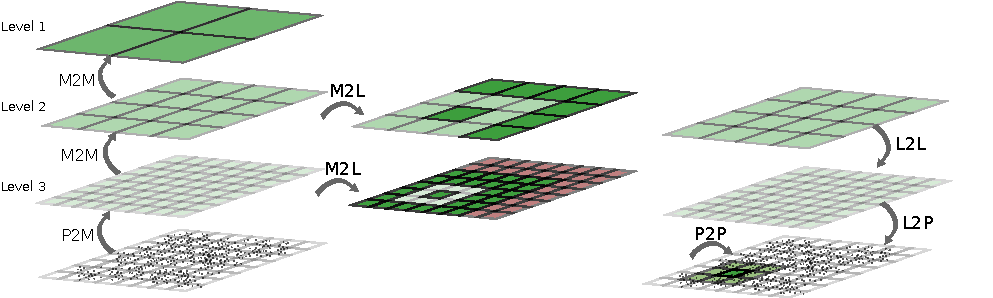
\includegraphics {figures/algorithm.pdf}}
\caption{The FMM illustrated for a two dimensional problem with a uniform octree. The left column illustrates the first two steps of the upward pass, beginning with the P2M operation to find the multipole expansions at the leaf level, followed by an M2M operation. The central and right columns illustrate the downward pass. In the central column, the far-field of a given box is highlighted, we observe that at level three the far field highlighted in red is already encapsulated in the local expansion of the given box due to the L2L translation from its parent. In the right column we see how the algorithm concludes with a given box evaluating it's near field of adjacent boxes, directly via the P2P operation.}
\label{fig:tree_traversal}
\end{figure*}

The $\mathcal{O}(N)$ algorithmic runtime complexity can be roughly seen to be the result of the ability to exactly translate between the multipole and local expansion representations for all boxes deemed to be in the far field of a given box, as well as the recursive procedure of the FMM. As a result of this, each box must only consider its interaction with a constant number of other boxes. As there are $\mathcal{O}(N)$ boxes in a given tree, the entire algorithm can be seen to be bounded by a runtime complexity of $\mathcal{O}(N)$.

The coefficients of a given multipole expansion are kernel-dependent in the sense that they will depend on the form of (\ref{eq:sec:intro:laplace_kernel}), software implementations have to be rewritten for each specific physical model. Fast multipole methods for generic kernel functions have been developed \cite{Gimbutas2003}, however there are fewer methods that rely only on numerical kernel evaluations, rather than analytic series expansions, examples include \cite{Fong2009, Ying2004}. The latter approaches are often referred to as kernel-independent fast multipole methods [KIFMM]. PyExaFMM utilizes the approach first presented by Ying et. al \cite{Ying2004}. This KIFMM represents the multipole expansions due to a cluster of charges as set of equivalent charge densities supported on a surface enclosing the cluster, with the fields generated by the charges are matched with an equivalent field generated by these equivalent densities via a least-squares fitting by considering their generated potential in the far field. As originally developed in \cite{Ying2004}, this method generalizes the FMM to non-oscillatory second-order elliptic partial differential equations with constant coefficients, for example the Laplace or Stokes equations. This includes many common problems, such as our model electrostatic problem. Further work has extended the method to include oscillatory problems, for example to solve the Helmholtz equation \cite{Engquist2007}.

At present, numerous high-quality open source implementations exist to solve FMM problems, both using analytic expansions for various kernels \cite{Gimbutas2010}, as well as using the KIFMM of Fong et. al \cite{Bramas2020}, \cite{Agullo2016}, and Ying et. al \cite{Wang2021}, \cite{Lashuk2012}. Some of these implementations are able to scale on supercomputing clusters, and solve problems involving millions of degrees of freedom \cite{Lashuk2012}. Others are designed to be run on a single workstation \cite{Bramas2020, Wang2021}. These softwares are developed in compiled languages, such as Fortran or C++, often making use of numerous non-standard libraries and language features. Compiled languages are often accompanied by complex build processes, making deployment to different platforms or architectures non-trivial. Many domain specialists who may want to use the FMM to aid their research, usually have limited computational skill sets, often restricted to subsets of Python, for data-analysis or simple numerical computing, or Matlab. Therefore it is not feasible for many users of to contribute to, or extend, many of these existing libraries without a significant investment in acquiring new skills. This problem is not unique to FMM implementations, but is general across high-performance computing [HPC] software.

In recent years, HPC libraries that aid in bypassing the limitations of the Python interpreter have emerged. The most pertinent example is Numba, a `just in time' [JIT] compiler for CPython, the most commonly used implementation of the Python interpreter written in the C language. JIT refers to the fact that the compiler waits until a Numba enhanced object, either a function or a class, is instantiated at runtime, before running optimizations to convert the Python source code into efficient machine code. Numba achieves performance by focussing solely on optimizing operations on the multi-dimensional array objects provided by Numpy, the ndarray. Numpy already provides a Python binding to HPC libraries that are written in C or Fortran, such as LAPACK and BLAS. Numba extends Numpy by removing inefficient layers of indirection for indexing into Numpy arrays, and instead translating array index operations into direct load and store operations from pointers \cite{Lam2015}. Furthermore, Numba is a `drop-in' library. It's simply installed via package manager, and objects are marked to be optimized by a single decorator. If Numba is unable to perform an optimization, it fails silently, deferring to the ordinary Python runtime. Therefore users are able to seamlessly incorporate Numba into new or existing projects. Previously, achieving similar behavior in Python would have required the usage of a hybrid language such as Cython, or by writing custom C extensions on top of Python code.

Numba has been extended with optimized versions of many common array operations, as well as common linear algebra routines available through the Numpy library. These are called automatically when used in a marked object. For common array operations, Numba is able to achieve comparable performance with compiled languages \cite{Lam2015}. Furthermore, Numba allows users to decorate functions to be run on GPUs, allowing for users to develop heterogenous applications from a single Python source. By using Numba in conjunction with Numpy, it is possible to achieve compiled-language performance for a variety of numerical problems from within Python.

Therefore, the question arises of whether it is feasible to develop a complex HPC application entirely within Python. The vision being that a domain specialist may be able to iterate from a prototype, to a high-performance application, using a language they are comfortable with. Python has the additional benefit of simple cross platform build tools, such as Conda, making it easy for developers to code once and deploy everywhere. An FMM implementation is an excellent case study to understand the maturity of Python for HPC development. As Numba is built to optimize operations on arrays, it represents a challenge to develop efficient representations and operations for the tree on which the algorithm is based. PyExaFMM was developed to answer the above question. It is currently a single node implementation designed for three-dimensional problems, implementing parallel strategies on multicore architectures, similar to \cite{Bramas2020, Wang2021}.

In developing PyExaFMM we demonstrate the feasibility of building a high-performance implementation of a non-trivial algorithm solely in Python. We achieve runtime performance within an order of magnitude of a comparable state of the art compiled language implementation. As with all Python applications, performance is degraded by portions of code that are unavoidably interpreted. However, this represents a compromise between usability and performance. Where by usability, we mean the ease by which non-software specialists can understand, alter, or extend the codebase to their needs. Using lines-of-code [LOC] as a rough metric of usability, PyExaFMM consists of approximately 3,300 LOC, compared with approximately 20,000 LOC and 50,000 LOC for the comparable C++ implementations, ExaFMM-T \cite{Wang2021} and TBFMM \cite{Bramas2020} respectively.

In this article we begin by providing an overview of the mathematical formulation behind the KIFMM in \cite{Ying2004}, before introducing Numba and discussing how it is used by PyExaFMM to accelerate computations, as well as program efficient data structures. We continue by discussing the mathematical and software based optimizations used by PyExaFMM for performance. Specifically how we efficiently pre-compute, cache, and apply FMM operations, and we provide an overview of the software design used in order to implement Numba optimizations effectively. We conclude with a discussion comparing the performance, in terms of accuracy, runtimes, and memory footprint, with the comparable state-of-the-art C++ implementation from the ExaFMM project, ExaFMM-T \cite{Wang2021}.

\section{THE KERNEL-INDEPENDENT FAST MULTIPOLE METHOD}

- Basic concept of matching potentials in the Far field
- Diagrams of operators.
- Interaction lists, and how these result from adaptivity.
- Concept of balanced octrees, and why they help with computing interaction lists
- Detail the complete algorithm
- List the difficulties in developing good KIFMMs (Ill Conditioning of c2e matrix, sparsification of the M2L operation)
- The most intensive computations are P2M and M2L, explain why.


\subsection{Algorithm}

\section{TECHNIQUES FOR ACHIEVING PERFORMANCE}

\subsection{What is Numba?}

What is does, how is it useful? Where do we use it, and why there. How much difference can it make in an idealized routine. What doesn't work, why doesn't it work. Where to be careful. Programming to an (invisible) framework \dots

Where is numba used heavily? Tree construction routines on Morton coordinates. Multithreading of tree construction, as well as P2M evaluation. Experiment to demonstrate the speed of kernel evaluation, with caveat that data must be pre-organised.

\subsection{Precomputing Operators}

Transfer vectors, hashing, HDF5, loading into memory.

\subsection{Compressing the M2L step with a randomised SVD}

Introduce \cite{Ying2004}. Numerical bounds on error out of scope, but show how experiments demonstrate that the FMM error dominates the SVD error.

\subsection{Software Architecture}

The key is separating routines to be accelerated, and organising data ready to run. The data organisation part (and it's slowness) should be demonstrated as a bottleneck using experiment.

\section{PERFORMANCE COMPARISON WITH STATE OF THE ART}

Description of main experiments, and how they are conducted. What are the main results? Are they expected from theory? What conclusions can be drawn about developing HPC codes entirely in Python, is it worth it?

% \begin{figure}
% \centerline{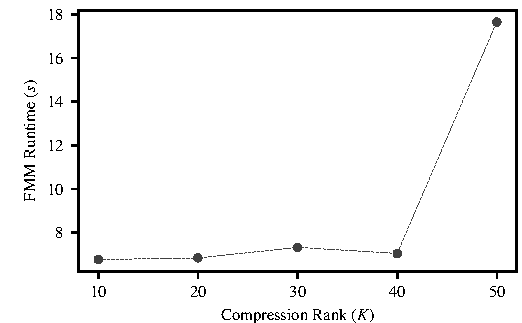
\includegraphics[width=18.5pc]{figures/compression_runtime.pdf}}
% \caption{Compression Rank and runtime}
% \end{figure}

% \begin{figure}
% \centerline{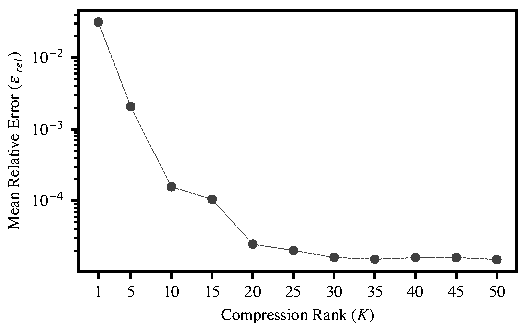
\includegraphics[width=18.5pc]{figures/compression_accuracy.pdf}}
% \caption{Compression Rank and accuracy}
% \end{figure}

% \begin{figure}
% 	\centerline{
\includegraphics[width=18.5pc]{figures/interaction_lists.pdf}}
% 	\caption{Compression Rank and accuracy}
% \end{figure}


% \begin{figure*}
% \centerline{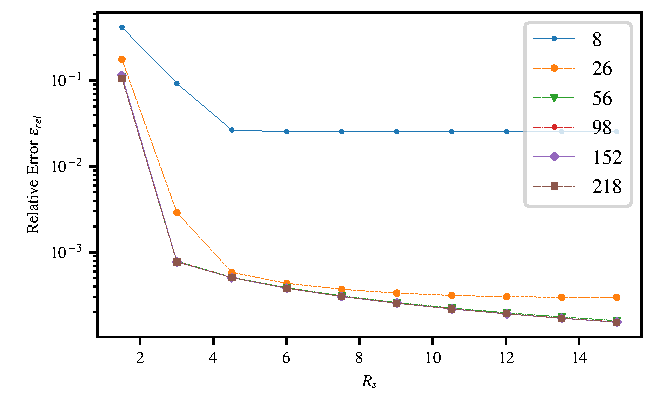
\includegraphics[width=26pc]{figures/pyexafmm_multipole_convergence.pdf}}
% \caption{PyExaFMM Multipole Expansion Convergence}
% \end{figure*}

% \begin{figure*}
% \centerline{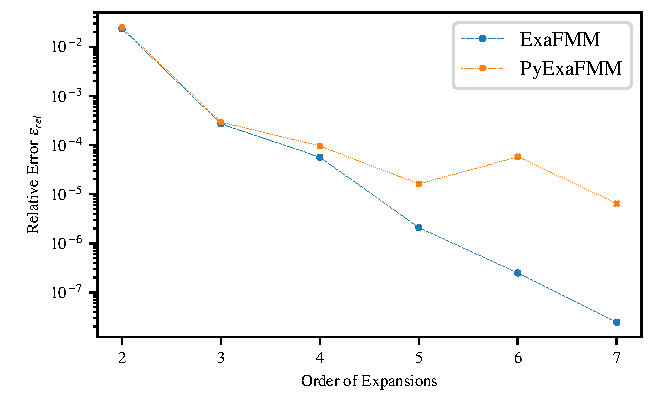
\includegraphics[width=26pc]{figures/potential_convergence.pdf}}
% \caption{Potential Convergence Comparison}
% \end{figure*}


% \begin{table}
% \caption{Units for magnetic properties.}
% \label{table}
% \small
% \begin{tabular*}{17.5pc}{@{}|p{29pt}|p{63pt}<{\raggedright}|p{80pt}<{\raggedright}|@{}}
% \hline
% Symbol&
% Quantity&
% Conversion from Gaussian and  CGS EMU to SI$^{\mathrm{a}}$ \\
% \hline
% $\Phi $&
% Magnetic flux&
% 1 Mx $\to  10^{-8}$ Wb $= 10^{-8}$ V $\cdot$ s \\
% $B$&
% Magnetic flux density,   magnetic induction&
% 1 G $\to  10^{-4}$ T $= 10^{-4}$ Wb/m$^{2}$ \\
% $H$&
% Magnetic field strength&
% 1 Oe $\to  10^{-3}/(4\pi )$ A/m \\
% $m$&
% Magnetic moment&
% 1 erg/G $=$ 1 emu   $\to 10^{-3}$ A $\cdot$ m$^{2} = 10^{-3}$ J/T \\
% $M$&
% Magnetization&
% 1 erg/(G $\cdot$ cm$^{3}) =$ 1 emu/cm$^{3}$   $\to 10^{-3}$ A/m \\
% 4$\pi M$&
% Magnetization&
% 1 G $\to  10^{-3}/(4\pi )$ A/m \\
% $\sigma $&
% Specific magnetization&
% 1 erg/(G $\cdot$ g) $=$ 1 emu/g $\to $ 1 A $\cdot$ m$^{2}$/kg \\
% $j$&
% Magnetic dipole   moment&
% 1 erg/G $=$ 1 emu   $\to 4\pi \times  10^{-10}$ Wb $\cdot$ m \\
% $J$&
% Magnetic polarization&
% 1 erg/(G $\cdot$ cm$^{3}) =$ 1 emu/cm$^{3}$  $\to 4\pi \times  10^{-4}$ T \\
% $\chi , \kappa $&
% Susceptibility&
% 1 $\to  4\pi $ \\
% $\chi_{\rho }$&
% Mass susceptibility&
% 1 cm$^{3}$/g $\to  4\pi \times  10^{-3}$ m$^{3}$/kg \\
% $\mu $&
% Permeability&
% 1 $\to  4\pi \times  10^{-7}$ H/m   $= 4\pi \times  10^{-7}$ Wb/(A $\cdot$ m) \\
% $\mu_{r}$&
% Relative permeability&
% $\mu \to \mu_{r}$ \\
% $w, W$&
% Energy density&
% 1 erg/cm$^{3} \to  10^{-1}$ J/m$^{3}$ \\
% $N, D$&
% Demagnetizing factor&
% 1 $\to  1/(4\pi )$ \\
% \hline
% \multicolumn{3}{@{}p{17.5pc}@{}}{Vertical lines are optional in tables. Statements that serve as captions for
% the entire table do not need footnote letters. }\\
% \multicolumn{3}{@{}p{17.5pc}@{}}{$^{\mathrm{a}}$Gaussian units are the same as cg emu for magnetostatics; Mx
% $=$ maxwell, G $=$ gauss, Oe $=$ oersted; Wb $=$ weber, V $=$ volt, s $=$
% second, T $=$ tesla, m $=$ meter, A $=$ ampere, J $=$ joule, kg $=$
% kilogram, H $=$ henry.}
% \end{tabular*}
% \label{tab1}
% \end{table}


\section{CONCLUSION}

What have we learned, what will we be working on next?

\section{ACKNOWLEDGMENT}

SK is supported by EPSRC Studentship 2417009.

\bibliography{pyexafmm}
\bibliographystyle{ieeetr}

\begin{IEEEbiography}{Srinath Kailasa}{\,} is a graduate student at University College London. He is currently pursuing a PhD in Computational Mathematics, having received an MPhys in Physics (2017) and an MSc Scientific Computing (2020) from the University of Durham, and University College London respectively. His research interests are in high-performance and scientific computing. Contact him at srinath.kailasa.18@ucl.ac.uk.
\end{IEEEbiography}

\begin{IEEEbiography}{Timo Betcke}{\,}is a Professor of Computational Mathematics at University College London. Contact him at t.betcke@ucl.ac.uk.
\end{IEEEbiography}

\begin{IEEEbiography}{Tingyu Wang}{\,}is a PhD student in Mechanical Engineering at the George Washington University. Contact him at twang66@email.gwu.edu.
\end{IEEEbiography}

\begin{IEEEbiography}{Lorena. A. Barba}{\,}is a Professor of Mechanical and Aerospace Engineering at the George Washington University.  Contact her at labarba@email.gwu.edu.
\end{IEEEbiography}

\end{document}

